\chapter{3DCityDB and Energy ADE Schema}
\label{app:citygml_schema}

This appendix presents the high-level schema architecture of 3DCityDB extended with the Energy Application Domain Extension (Energy ADE), illustrating the mapping between CIM Wizard data structures and the CityGML standard. Figure~\ref{fig:citygml_schema} provides an overview of the schema components and their relationships.

\begin{figure}[htbp]
\centering
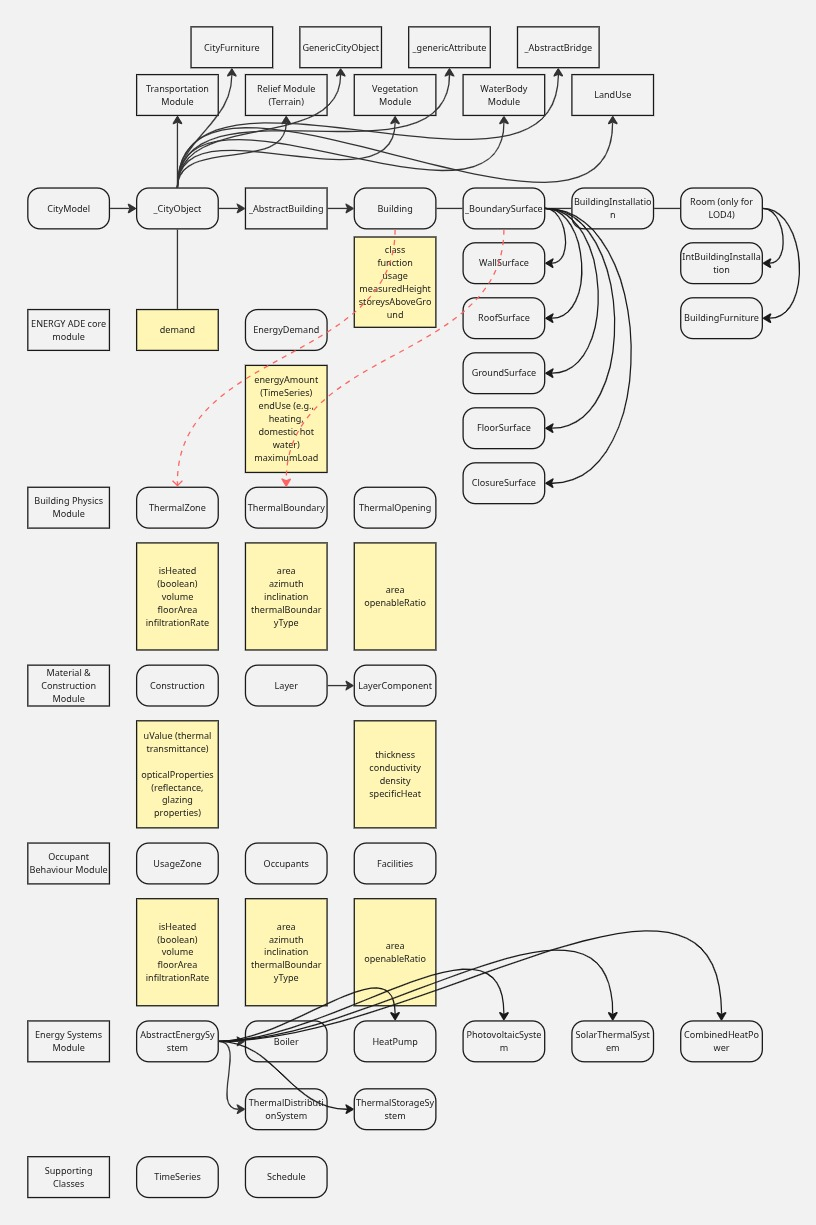
\includegraphics[width=0.95\textwidth]{Figures/citygml.jpg}
\caption{High-level schema of 3DCityDB with Energy ADE extension showing the mapping from CIM Wizard to CityGML. Each CIM Wizard scenario maps to a CityModel, buildings map to CityObject instances, and TABULA-derived attributes populate the Energy ADE thermal and system properties.}
\label{fig:citygml_schema}
\end{figure}

\section{Schema Mapping Overview}

The integration between CIM Wizard and 3DCityDB follows a hierarchical mapping structure that preserves semantic relationships while enabling interoperability with CityGML-compliant tools and simulation platforms.

\subsection{CityModel Level (Scenario Mapping)}

Each CIM Wizard \textbf{scenario} corresponds to a \texttt{CityModel} in 3DCityDB. The CityModel serves as the root container for all urban objects within a specific analysis context, enabling:
\begin{itemize}[leftmargin=1.2em]
    \item Scenario-based organization where baseline, optimized, and future configurations exist as separate CityModels
    \item Temporal versioning through CityModel metadata attributes
    \item Coordinate reference system (CRS) specification for spatial consistency
    \item Envelope bounds defining the geographic extent of the study area
\end{itemize}

\subsection{CityObject Level (Building Mapping)}

Each CIM Wizard \textbf{building} maps to a \texttt{Building} CityObject within the CityModel hierarchy. The Building class in CityGML/3DCityDB provides:
\begin{itemize}[leftmargin=1.2em]
    \item \texttt{gml:id} -- Unique identifier linked to CIM Wizard \texttt{building\_id}
    \item \texttt{bldg:yearOfConstruction} -- Construction period from census/TABULA classification
    \item \texttt{bldg:measuredHeight} -- Building height from DSM-DTM calculation
    \item \texttt{bldg:storeysAboveGround} -- Floor count from height-based estimation
    \item \texttt{bldg:function} -- Usage type (residential, commercial, mixed)
    \item Geometric representation at appropriate Level of Detail (LoD 1.2 for CIM Wizard)
\end{itemize}

\subsection{Energy ADE Extensions}

The Energy ADE extends the base CityGML schema with thermal and energy system attributes populated from TABULA archetypes:

\paragraph{ThermalBoundary and ThermalComponent}
Building envelope surfaces (\texttt{WallSurface}, \texttt{RoofSurface}, \texttt{GroundSurface}) are linked to \texttt{ThermalBoundary} objects containing:
\begin{itemize}[leftmargin=1.2em]
    \item \texttt{thermalBoundaryType} -- Surface classification (wall, roof, floor, window)
    \item \texttt{area} -- Surface area computed from LoD 1.2 geometry
    \item \texttt{azimuth} and \texttt{inclination} -- Orientation parameters
    \item \texttt{ThermalComponent} references with U-values from TABULA lookup
\end{itemize}

\paragraph{Construction and Material}
The \texttt{Construction} class stores layered material compositions:
\begin{itemize}[leftmargin=1.2em]
    \item \texttt{Layer} objects representing material strata with thickness
    \item \texttt{Material} properties including thermal conductivity and density
    \item Reference to TABULA construction type identifiers
\end{itemize}

\paragraph{EnergyConversionSystem}
Heating, cooling, and domestic hot water systems from TABULA archetypes map to:
\begin{itemize}[leftmargin=1.2em]
    \item \texttt{conversionSystemType} -- System classification (boiler, heat pump, etc.)
    \item \texttt{efficiencyIndicator} -- System efficiency or COP
    \item \texttt{energyCarrier} -- Fuel type (gas, electricity, oil)
    \item \texttt{nominalPower} -- Rated capacity
\end{itemize}

\section{Data Flow Summary}

The complete data flow from CIM Wizard to 3DCityDB Energy ADE proceeds as follows:

\begin{enumerate}[leftmargin=1.2em]
    \item \textbf{Scenario Creation}: CIM Wizard project boundary defines the CityModel envelope
    \item \textbf{Building Import}: GeoJSON footprints or OSM data create Building CityObjects
    \item \textbf{Geometry Enrichment}: Height calculation enables LoD 1.2 extrusion with semantic surfaces
    \item \textbf{TABULA Classification}: Construction period and building type determine archetype
    \item \textbf{Attribute Population}: U-values, system parameters, and WWR from TABULA tables
    \item \textbf{Energy ADE Storage}: Thermal boundaries, constructions, and systems persisted to 3DCityDB
    \item \textbf{Export}: CityJSON/CityGML output for simulation tool integration
\end{enumerate}

This systematic mapping ensures that CIM Wizard's sparse input data is transformed into semantically rich, standards-compliant city models suitable for urban energy simulation and analysis.

